\documentclass[english,compress]{beamer}
% {{{ preamble
%\batchmode
\usepackage{kloeckislides}
\nonstopmode

\usepackage{pifont}

\useoutertheme{split}
\useinnertheme{rectangles}
\usecolortheme{uiuc}
\usetikzlibrary{arrows}

\usepackage{ifthen}

\pgfdeclareimage[height=0.8cm]{uiuc-logo}{uiuc-logo.pdf}
\def\mylogotext{\pgfuseimage{uiuc-logo}\hspace*{0.3cm}}
%\def\mylogotext{}

\AtBeginSection[] {
  \begin{frame}<beamer>
  \frametitle{Outline}
  \tableofcontents[sectionstyle=show/shaded,subsectionstyle=show/show/hide]
\end{frame}
}
\AtBeginSubsection[] {
  \begin{frame}<beamer>
  \frametitle{Outline}
  \tableofcontents[sectionstyle=show/shaded,subsectionstyle=show/shaded/hide]
\end{frame}
}

\definecolor{green}{RGB}{0, 180, 0}
\definecolor{red}{RGB}{180, 0, 0}
\colorlet{grellow}{green!50!yellow}
\colorlet{codeback}{gray!20}

\DeclareMathOperator{\argmin}{argmin}
\DeclareMathOperator{\argmax}{argmax}


\lstset{
  language=Python,
  alsolanguage=C,
  rangebeginprefix=\#\ ,
  rangeendprefix=\#\ ,
  }

\colorlet{input}{green!30}
\colorlet{output}{red!30}
\colorlet{intermed}{blue!30}

\definecolor{fetch}{RGB}{227,110,35}
\definecolor{alu}{RGB}{255,188,24}
\definecolor{context}{RGB}{132,146,175}


\setbeamertemplate{navigation symbols}{}

\let\tmop=\operatorname

\usepackage[normalem]{ulem}

\def\curl{\operatorname{curl}}

\def\checkmark{\textbf{\color{green}\ding{51}}}
\def\crossmark{\textbf{\color{red}\ding{56}}}


\logoenable

\pgfdeclarelayer{grid}
\pgfsetlayers{background,grid,main,foreground}
\def\intd{\, d}

\tikzset{%
  input/.style={circle,fill=input,draw,thick,minimum height=4.5ex},
  output/.style={circle,fill=output,draw,thick,minimum height=4.5ex},
  func/.style={->,thick},
}
\def\bigncentered#1{
  \begin{center}
    \Huge\bfseries #1
  \end{center}
}
\def\weblink#1#2{\href{#1}{\color{blue}\underline{#2}}}

\begin{document}

% -----------------------------------------------------------------------------
% {{{ front matter
% -----------------------------------------------------------------------------

\title{Part 3: OpenCL}

\author{Andreas Klöckner}

\institute[Computer Science $\cdot$ UIUC]
{Computer Science\\University of Illinois at Urbana-Champaign}

\date{}

\frame{
  \titlepage
}
% }}}
% -----------------------------------------------------------------------------
\section{OpenCL}
% -----------------------------------------------------------------------------
% {{{
\begin{frame}{What is OpenCL?}
  \begin{columns}
    \column{0.7\textwidth}

      OpenCL (Open Computing Language) is an open, royalty-free
      standard for general purpose parallel programming across CPUs,
      GPUs and other processors.
      \hfill{\footnotesize[OpenCL 1.1 spec]}
      \bigskip


      \begin{itemize}
        \item Device-neutral (Nv GPU, AMD GPU, Intel/AMD CPU)
        \item Vendor-neutral
        \item Comes with RTCG
      \end{itemize}
      Defines:
      \begin{itemize}
        \item Host-side programming interface (library)
        \item Device-side programming language (!)
      \end{itemize}

    \column{0.3\textwidth}
      
\includegraphics[width=\textwidth] {opencl-logo.png}

  \end{columns}
\end{frame}


\newcommand{\khronoscredit}{
  \begin{tikzpicture}[overlay]
    \node [xshift=1cm,yshift=0.5cm]
      at (current page.south west)
      [font=\scriptsize,fill=gray!30,anchor=south west,opacity=0.5]
      {Credit: Khronos Group};
  \end{tikzpicture}
}
\def\khronosslide#1#2
{
  \begin{frame}{#1}
    \hspace*{-0.75cm}
\includegraphics[viewport=2cm 0cm 31cm 14.5cm,clip=true,width=1.15\textwidth,page=#2]{opencl-overview.pdf}
    \khronoscredit
  \end{frame}
}
\begin{nologo}
\khronosslide{Who?}{4}
%\khronosslide{When?}{5}
\khronosslide{Why?}{3}
\end{nologo}


\begin{comment}
\begin{nologo}
\begin{frame}{CL vs CUDA side-by-side}
  \begin{columns}
    \column{0.5\textwidth}
      CUDA source code:
      \lstinputlisting[basicstyle=\tiny]{transpose.cu}
    \column{0.5\textwidth}
      OpenCL source code:
      \lstinputlisting[basicstyle=\tiny]{transpose.cl}
  \end{columns}
\end{frame}
\end{nologo}
\end{comment}

%\begin{frame}{OpenCL $\leftrightarrow$ CUDA: A dictionary}
  \begin{tikzpicture}[overlay]
    \node [anchor=south east,rotate=10,opacity=0.3] 
    at ($(current page.south east) + (-0.5cm,2cm)$)
    { \includegraphics[width=6cm]{dictionary-desat.jpeg} } ;
  \end{tikzpicture}

  \begin{tabular}{r|l}
    \textbf{OpenCL} & \textbf{CUDA} \\
    \hline
    Grid & Grid \\
    Work Group& Block \\
    Work Item & Thread \\
    \texttt{\_\_kernel} & \texttt{\_\_global\_\_} \\
    \texttt{\_\_global} & \texttt{\_\_device\_\_} \\
    \texttt{\_\_local} & \texttt{\_\_shared\_\_} \\
    \texttt{\_\_private} & \texttt{\_\_local\_\_} \\
    \texttt{image$n$d\_t} & \texttt{texture\textless type, $n$, ...\textgreater} \\
    \texttt{barrier(LMF)} & \texttt{\_\_syncthreads()} \\
    \texttt{get\_local\_id(012)} & \texttt{threadIdx.xyz} \\
    \texttt{get\_group\_id(012)} & \texttt{blockIdx.xyz} \\
    \texttt{get\_global\_id(012)} & -- (reimplement) \\
  \end{tabular}
\end{frame}
\addimgcredit{Dictionary: sxc.hu/topfer}

{
\def\evalprint#1{{\pgfmathtruncatemacro{\mathresult}{#1}\mathresult}}
\begin{frame}{OpenCL: Computing as a Service}

  \begin{tikzpicture}[
    z={(0.5cm,-1cm)},
    every shadow/.style={shadow xshift=-0.1cm,shadow yshift=0.1cm},
    memory/.style={fill=blue!40,draw=blue},
    langarrow/.style={single arrow,shape border rotate=90,
      single arrow tip angle=165,single arrow head extend=0.6cm,
      draw,thick,fill=yellow},
  ]
    \uncover<+->{
    \node [draw,inner sep=5mm,fill=green!40,drop shadow,
      text width=1.5cm,text centered] (host) {Host\\(CPU)} ;
      \uncover<3-4>{
        \node [above left=0.2cm of host.south east,font=\tiny,memory,
          inner sep=0.5mm,minimum width=1.3cm]
          { Memory } ;
      }
    }
    \uncover<+->{
      \foreach \i in {0,...,3}
      {
        \pgfmathtruncatemacro{\plat}{\i/2}
        \node 
          [draw,fill=yellow!50, anchor=west,text width=4.5cm,font=\small] 
          at ($(host.east)+(1.75+\plat,0,-1.5+\i)$)
          (cdev\i)
          {
            Compute Device \evalprint{mod(\i,2)}
            {\tiny(Platform \evalprint{\i/2})}\\
            \begin{tikzpicture}
              \foreach \j in {0,1,2}
              {
                \foreach \k in {0,1,2,7}
                  \coordinate (pe\i\j\k) at (0.15*\k,0,0.2*\j) ;
                \node 
                  [draw,fill=orange!40,fit={(pe\i\j0) (pe\i\j7) (0,0.4,0.2*\j) }] 
                  (unit\i\j)
                  {};
                \foreach \k in {0,1,2,7}
                  \filldraw 
                    [fill=red!30]
                    (pe\i\j\k) ++(-0.05,0) rectangle ++ (0.1,0.4) ;
                \node at (4.5*0.15,0.2,0.2*\j) 
                  [anchor=center,font=\tiny,text width=] 
                  {$\cdots$} ;
              }
              \uncover<4>{
                \draw (pe\i27) ++(0.5,0) 
                  node [anchor=south west,memory,text width=,minimum height=0.8cm]
                  {Memory};
              }
            \end{tikzpicture}
          } ;
        \draw [thick] 
          (host.east) -- ++(1,0) -- ++(0,0,-1.5+\i) -- ++(\plat+0.75,0);
      }
    }

    % memory ------------------------------------------------------------------
    \uncover<+>{}
    \uncover<+>{}

    % platforms ---------------------------------------------------------------
    \uncover<+>{}
    \uncover<+>{
      \node [fit=(cdev0) (cdev1),draw,dashed,thick] (plat0) {} ;
      \node at (plat0.north west) [anchor=south west]
        {Platform 0 (e.g. CPUs)} ;
    }
    \uncover<+>{
      \node [fit=(cdev2) (cdev3),draw,dashed,thick] (plat1) {} ;
      \node at (plat1.south west) [anchor=north west]
        {Platform 1 (e.g. GPUs)} ;
    }

    % hardware ----------------------------------------------------------------
    \uncover<+>{}
    \uncover<+-+(2)>{
      \draw [<-,thick] (cdev0) -- ++(-3,0.35)
        node [anchor=east,text width=2.5cm] 
          {(think ``chip'',\\ has memory interface)} ;
    }
    \uncover<+-+(1)>{
      \draw [<-,thick] (unit32.center) -- ++(-3,0.1)
        node [anchor=east,text width=3.25cm] 
          {Compute Unit\\(think ``processor'',\\ has insn. fetch)} ;
    }
    \uncover<+>{
      \draw [<-,thick] (pe327) -- ++(-1.5,-1)
        node [anchor=east,text width=3.35cm] 
          {Processing Element\\(think ``SIMD lane'')} ;
    }

    % programming interfaces --------------------------------------------------
    \uncover<+>{}
    \uncover<+-+(1)>{
      \node [fit=(host)] (hostwrap) {} ;
      \node at (hostwrap.south) 
        [anchor=north,langarrow]
        {Python} ;
    }
    \uncover<+->{
      \node [fit=(plat0) (plat1)] (devwrap) {} ;
      \node at (devwrap.south) 
        [anchor=north,draw,langarrow]
        {Device Language: $\sim$ C99} ;
    }
  \end{tikzpicture}
\end{frame}
}

%\begin{frame}{OpenCL: Execution Model}
  \begin{columns}
  \column{.3\textwidth}
    \begin{tikzpicture}[font=\tiny\bfseries,y=-1cm,anchor=north west]
      \node at (0,-0.4) [inner sep=0] (gridtitle) {$n$D Grid};
      \foreach \x in {0, 1, 2}
        \foreach \y in {0, 1}
          \node at (0.9*\x, 0.75*\y ) (wgroup\x\y) [draw, fill=red!60, rectangle, 
            text width=0.6cm, text centered, inner sep=1mm]
              {Group $(\x, \y)$} ;

      \begin{pgfonlayer}{background}
        \node [draw,thick,fill=red!30,fit=(gridtitle) (wgroup21)] (gridbox) {} ;
      \end{pgfonlayer}

      \begin{scope}[yshift=-3cm]
      \node at (0, -0.4) [inner sep=0] (grouptitle) {Work Group $(1,0)$};
      \foreach \x in {0, 1, 2, 3}
        \foreach \y in {0, 1, 2, 3}
          \node at (0.8*\x, .75*\y) [draw, fill=red!90, rectangle, text width=0.5cm, 
            text centered,inner sep=1mm]
            (item\x\y) { Item $(\x, \y)$ };
      \end{scope}

      \begin{pgfonlayer}{background}
        \node [draw,thick,fill=red!60,fit=(grouptitle) (item33)] (groupbox) {} ;
      \end{pgfonlayer}

      \draw[dashed] (wgroup11.south west) -- (groupbox.north west);
      \draw[dashed] (wgroup11.south east) -- (groupbox.north east);

    \end{tikzpicture}

  \column{0.7\textwidth}

    \begin{itemize}
      \item<+-> Two-tiered Parallelism
        \begin{itemize}
        \item Grid = $N_x\times N_y \times N_z$ work groups
        \item Work group = $S_x \times S_y\times S_z$ work items
        \item Total: $\prod_{i\in\{x,y,z\}} S_i N_i$ work items
        \end{itemize}
      \item<+-> Comm/Sync only within work group
        \begin{itemize}
        \item Work group maps to compute unit
        \end{itemize}
      \item<+-> Grid/Group $\approx$ outer loops in an algorithm
      \item<.-> Device Language:\\
        \texttt{get\_\{global,group,local\}\_\{id,size\}\\(\texttt{axis})}
    \end{itemize}
  \end{columns}
\end{frame}

%\begin{frame}{Why do Scripting for GPUs?}
  \begin{columns}
    \column{0.6\textwidth}
    \begin{itemize}
      \item GPUs are everything that scripting languages are not.
        \begin{itemize}
          \item Highly parallel
          \item Very architecture-sensitive
          \item Built for maximum FP/memory throughput
        \end{itemize}
        $\rightarrow$ complement each other
      \item CPU: largely restricted to control tasks ($\sim$1000/sec)
        \begin{itemize}
          \item Scripting fast enough
        \end{itemize}
      \item Python + CUDA = \textbf{PyCUDA}
      \item Python + OpenCL = \textbf{PyOpenCL}
    \end{itemize}
    \column{0.4\textwidth}
      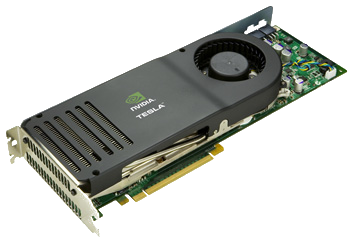
\includegraphics[width=\textwidth]{c870.png}
  \end{columns}
\end{frame}
\addimgcredit{C870 GPU: Nvidia Corp.}


\def\simplesm{{
  \node (fetch) [blk,fill=fetch] at (0,0) {Fetch/ Decode} ;
  \begin{scope}[yshift=-1.25cm]
  \foreach \x in {0,1,2,3}
  \foreach \y in {1,0}
  \draw [fill=alu,thick] (0.625*\x,0.5*\y) rectangle +(0.625,0.5);
  \end{scope}
  \node (pvt) [blk,fill=context, minimum height=2cm,below=1.5cm of fetch]
  {32 kiB Ctx Private (``Registers'') };
  \node (shared) [blk,fill=context,minimum height=1cm,below=0.2cm of pvt]
  {16 kiB Ctx Shared };
}}
\def\drawprocassign#1#2#3{
  \pgfmathtruncatemacro{\gj}{#1/4}
  \pgfmathtruncatemacro{\gi}{#1-\gj*4}
  \pgfmathtruncatemacro{\si}{#2/3}
  \pgfmathtruncatemacro{\sj}{#2-\si*3}
  \draw [->,ultra thick,#3] (g\gi\gj) ++(0.5,-0.5) ..controls +(0.3,1.2-0.2*\gi) and +(-0.5,0.5).. (sm\sj\si) ;
}
\begin{frame}{Connection: Hardware $\leftrightarrow$ Programming Model }
  \hspace*{-3mm}
  \begin{tikzpicture}[
  blk/.style={draw,thick,text centered,anchor=south west,minimum width=2.5cm,text width=2cm,font=\small},
  ]
    \uncover<+-+(3)>{
      \simplesm
    }
    \uncover<+->{
      \begin{scope}[xshift=8cm]
        \draw [thick,fill=black!20] (-0.5,0.5) rectangle +(3.5,-5.5)
        coordinate (hwboxse);

        \foreach \i in {0,1,2}
        \foreach \j in {0,1,2}
        {
          \node at (\i,-\j*1.75) (sm\i\j) {
            \begin{tikzpicture}[transform canvas={scale=0.25}]
              \simplesm
            \end{tikzpicture}
          };
        }
      \end{scope}
    }

    \uncover<+>{
      \node (smcircle) [circle,thick,draw,yshift=-0.45cm,xshift=0.3125cm,minimum
      height=1.8cm] at (sm02) {};

      \draw [line width=0.2ex,->] (smcircle) -- +(-4,1);
    }

    \uncover<+>{ % single core disappears
    }
    \uncover<+-+(2)>{
        \node [rotate=20,font=\Large\bfseries,
        cloud,cloud ignores aspect=true,cloud puffs=15,draw,thick,
        text width=4cm, text centered,anchor=north
        west,xshift=1cm,yshift=-1.25cm]
        {Who cares how many cores? };
    }
    \uncover<+-+(1)>{ 
      \node [anchor=west,draw,drop shadow,fill=white,
      text width=0.5\textwidth, inner xsep=0.5cm,inner ysep=0.5cm,thick]
      (prog-model-idea)
      at (0,-4cm)
        {
          Idea:

          \begin{itemize}
            \item Program as if there were ``infinitely'' many cores
            \item Program as if there were ``infinitely'' many ALUs per core
          \end{itemize}
        } ;
    }
    \uncover<+>{
      \node [anchor=north west,xshift=0.3cm,yshift=-0.6cm, draw,drop shadow,fill=white,
      text width=0.8\textwidth, inner xsep=0.5cm,inner ysep=0.5cm,thick]
      at (prog-model-idea.north west)
        {
          Consider: Which is easy to do automatically?
          \begin{itemize}
            \item Parallel program $\rightarrow$ sequential hardware
          \end{itemize}
          or
          \begin{itemize}
            \item Sequential program $\rightarrow$ parallel hardware?
          \end{itemize}

        } ;
    }
    \uncover<+>{ % notes disappear
    }
    \uncover<+->{
      \draw [thick,|->] (0,0.3) -- ++(3,0) 
        node [anchor=west,font=\small] { Axis 0 };
      \draw [thick,|->] (-0.3,0) -- ++(0,-2) 
        node [anchor=east,font=\small,rotate=90] { Axis 1 };

      \foreach \gi in {0,1,2,3}
        \foreach \gj in {0,1,2}
        {
          \draw [very thick,fill=black!20] (\gi*1.75,\gj*-1.5) coordinate (g\gi\gj)
            rectangle +(1.75,-1.5) ;
          \foreach \li in {1,2,3,4,5,6}
            \draw (g\gi\gj) ++(0.25*\li,0) -- +(0,-1.5) ;
          \foreach \li in {1,2,3,4,5}
            \draw (g\gi\gj) ++(0,-0.25*\li) -- +(1.75, 0) ;
        }
    }
    \coordinate (gridcenter) at (3,-2.25);
    \uncover<+->{
      \node [below=1.5cm of sm12,font=\Large] (hwlabel) { Hardware };
    }
    \uncover<+->{
      \node [below=2.5cm of gridcenter,font=\Large] (swreplabel)
      { Software representation };
    }
    \only<+-+(2)>{
      \node [font=\huge\bfseries,rotate=10, text width=5cm] at (3,-2.25) { Grid 

      (Kernel: Function on Grid) };
    }
    \only<+-+(1)>{
      \fill [black,opacity=0.3] (g00) rectangle (g11) ;
      \node [font=\Large\bfseries,anchor=north west] at (g10) { (Work) Group};
    }
    \only<+>{
      \fill [black,opacity=0.3] (g32) ++(0.5,-0.25) rectangle +(0.25,-0.25)
      node [pos=0.5] (workitem) {};
      \node [draw,thick,fill=white,font=\Large\bfseries,below=0.25 of
        workitem, arrow box, arrow box arrows={north:0.5cm}] { (Work) Item};
    }
    \only<+>{}
    \uncover<+>{
      \draw [<->,line width=1mm] (gridcenter)
      ..controls +(1,1) and +(-1,1)..
      (sm11)
      node [pos=0.6,anchor=south,yshift=0.5cm,font=\fontsize{40}{30}\bfseries] {?};
    }
    \only<+>{
      \fill [black,opacity=0.3] (g00) rectangle (g11) ;
      \drawprocassign{0}{0}{}
    }
    \only<+>{ \foreach \gnum in {0,1,2} { \drawprocassign{\gnum}{\gnum}{} } }
    \only<+>{ \foreach \gnum in {0,1,...,8} { \drawprocassign{\gnum}{\gnum}{} } }
    \only<+>{ \foreach \gnum in {0,1,...,8} { \drawprocassign{\gnum}{\gnum}{opacity=0.2} } }
    \only<+>{
      \foreach \gnum in {0,1,...,8}
      {
        \drawprocassign{\gnum}{\gnum}{opacity=0.2}
        \pgfmathtruncatemacro{\gj}{\gnum/4}
        \pgfmathtruncatemacro{\gi}{\gnum-\gj*4}
        \foreach \id in {0,...,7}
        {
          \pgfmathtruncatemacro{\li}{\id/7}
          \pgfmathtruncatemacro{\lj}{\id-\li*7}
          \fill [black,opacity=0.3]
            (g\gi\gj) ++ (0.25*\lj,-0.25*\li) rectangle +(0.25,-0.25);
        }
      }
    }
    \only<+>{
      \foreach \gnum in {0,1,...,8}
      {
        \drawprocassign{\gnum}{\gnum}{opacity=0.2}
        \pgfmathtruncatemacro{\gj}{\gnum/4}
        \pgfmathtruncatemacro{\gi}{\gnum-\gj*4}
        \foreach \id in {8,...,15}
        {
          \pgfmathtruncatemacro{\li}{\id/7}
          \pgfmathtruncatemacro{\lj}{\id-\li*7}
          \fill [black,opacity=0.3]
            (g\gi\gj) ++ (0.25*\lj,-0.25*\li) rectangle +(0.25,-0.25);
        }
      }
    }
    \only<+-+(2)>{
      \foreach \gnum in {0,1,...,8}
      {
        \drawprocassign{\gnum}{\gnum}{opacity=0.2}
        \pgfmathtruncatemacro{\gj}{\gnum/4}
        \pgfmathtruncatemacro{\gi}{\gnum-\gj*4}
        \foreach \id in {16,...,23}
        {
          \pgfmathtruncatemacro{\li}{\id/7}
          \pgfmathtruncatemacro{\lj}{\id-\li*7}
          \fill [black,opacity=0.3]
            (g\gi\gj) ++ (0.25*\lj,-0.25*\li) rectangle +(0.25,-0.25);
        }
      }
    }
    \uncover<+>{
        \node [above left=1cm of current page.south east, draw,drop shadow,fill=white,
        text width=0.4\textwidth, inner xsep=0.5cm,inner ysep=0.5cm,thick]
          {
            Really: Group provides pool of concurrency to draw from.

            \medskip
            X,Y,Z order \emph{within} group matters. (Not \emph{among}
            groups, though.)
          } ;
    }
    \only<+>{}
    \only<+>{ \foreach \gnum in {9,10,11} { \drawprocassign{\gnum}{(\gnum-9)}{} } }
    \only<+->{
      \fill [black,opacity=0.3] (g20) ++(+0.75,-0.25) rectangle ++(0.25,-0.25)
      coordinate [pos=0.5] (workitem2);
      \node [draw,thick,fill=white,below=0.25 of
        workitem2, arrow box, arrow box arrows={north:0.5cm},text width=0.85\textwidth] { 
          \begin{itemize}
            \item \texttt{get\_local\_id(axis)?/size(axis)?}
            \item \texttt{get\_group\_id(axis)?/num\_groups(axis)?}
            \item \texttt{get\_global\_id(axis)?/size(axis)?}
          \end{itemize}
          \texttt{axis=0,1,2,\dots}
        };
    }
  \end{tikzpicture}

  % ---------------------------------------------------------------------------
  \uncover<+>{%
    \begin{tikzpicture} [overlay]
      \node [below right=1cm of current page.north west, draw,drop shadow,fill=white,
      text width=0.6\textwidth, inner xsep=0.5cm,inner ysep=0.5cm,thick]
        {
          Grids can be 1,2,3-dimensional.
        } ;
    \end{tikzpicture}%
  }
\end{frame}



% }}}
% -----------------------------------------------------------------------------
\section{PyOpenCL}
% -----------------------------------------------------------------------------
% {{{
\begin{frame}
  \bigncentered{DEMO TIME}
\end{frame}
% }}}
% -----------------------------------------------------------------------------
\section[Patterns]{Parallel patterns}
% -----------------------------------------------------------------------------
\subsection{Map}
% -----------------------------------------------------------------------------
% {{{
\begin{frame}{Map}
  \uncover<+>{}
  {\Huge
  \[
    y_i = f_i(x_i)
  \]}%
  where $i\in\{1,\dots,N\}$.

  \medskip
  Notation: (also for rest of this lecture)
  \begin{itemize}
    \item $x_i$: inputs
    \item $y_i$: outputs
    \item $f_i$: (pure) functions (i.e. \emph{no side effects})
  \end{itemize}

  \medskip
  \uncover<+>{
    \begin{tikzpicture} [overlay]
      \node [below left=1cm of current page.north east, draw,drop shadow,fill=white,
      text width=0.75\textwidth, inner xsep=0.5cm,inner ysep=0.5cm,thick]
        {
          When does a function have a ``side effect''?

          \bigskip
          In addition to producing a value, it 
          \begin{itemize}
          \item modifies non-local state, or
          \item has an observable interaction with the outside world.
          \end{itemize}
        } ;
    \end{tikzpicture}
  }%
  \uncover<+(1)->{
  Often: $f_1=\dots=f_N$. Then
  \begin{itemize}
    \item Python function \texttt{map}
    %\item C++ STL \texttt{std::transform}
  \end{itemize}
  }
\end{frame}
% -----------------------------------------------------------------------------
\begin{frame}{Map: Graph Representation}
  \begin{center}
    \begin{tikzpicture}
      \foreach \i in {0,1,...,8}
      {
        \node [input] at (\i, 0) (x\i) { $x_{\i}$ };
        \node [output] at (\i, -2) (y\i) { $y_{\i}$ };
        \draw [func] (x\i) -- (y\i) node [pos=0.5,anchor=east] {$f_{\i}$};
      }
    \end{tikzpicture}
  \end{center}
  \uncover<2>{
    \begin{tikzpicture} [overlay]
      \node [above left=1cm of current page.south east, draw,drop shadow,fill=white,
      text width=0.4\textwidth, inner xsep=0.5cm,inner ysep=0.5cm,thick]
        {
          Trivial? Often: no.
        } ;
    \end{tikzpicture}
  }
\end{frame}
% -----------------------------------------------------------------------------
\begin{frame}{Embarrassingly Parallel: Examples}
  \begin{columns}
    \column{0.6\textwidth}
      Surprisingly useful:
      \begin{itemize}
        \item Element-wise linear algebra: 

          Addition, scalar
          multiplication (\emph{not} inner product)
        \item Image Processing: Shift, rotate, clip, scale, \dots
        \item Monte Carlo simulation
        \item (Brute-force) Optimization
        \item Random Number Generation
        \item Encryption, Compression

          (after blocking)
        %\item Software compilation
          %\subitem{\texttt{make -j8}}
      \end{itemize}
    \column{0.4\textwidth}
      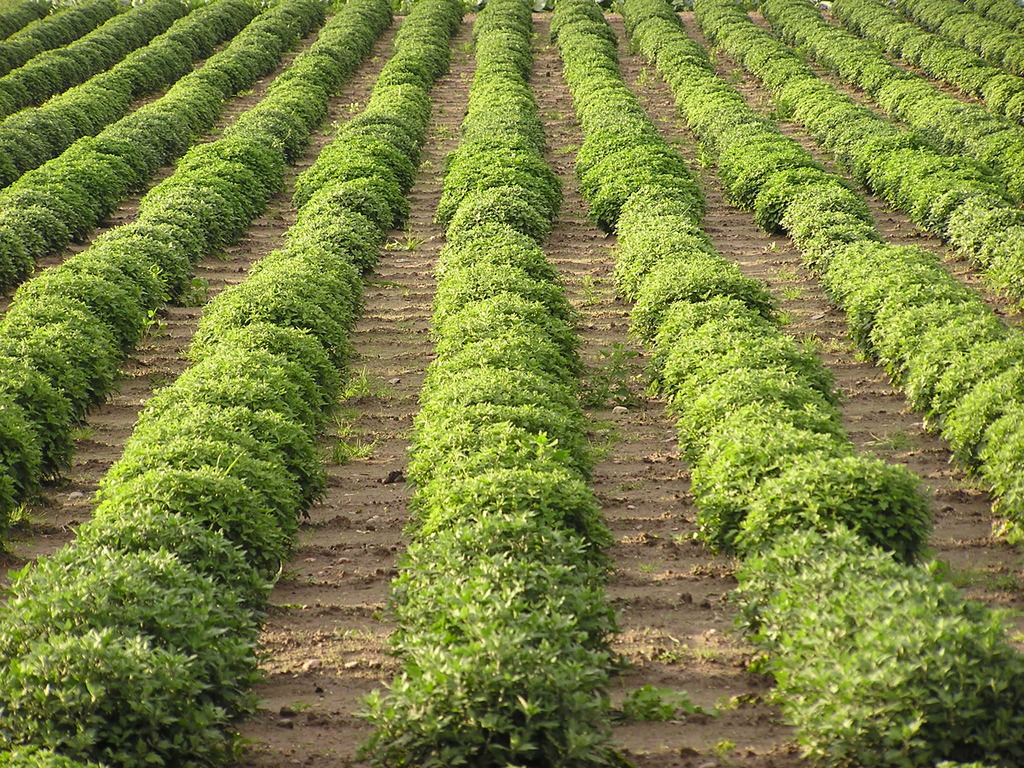
\includegraphics[width=\textwidth]{parallel-field.jpeg}
  \end{columns}
  % \uncover<2>{
  %   \begin{tikzpicture} [overlay]
  %     \node [above left=1cm of current page.south east, draw,drop shadow,fill=white,
  %     text width=0.5\textwidth, inner xsep=0.5cm,inner ysep=0.5cm,thick]
  %       {
  %         But: Still needs a minimum of coordination. How can that be
  %         achieved?
  %       } ;
  %   \end{tikzpicture}
  % }
\end{frame}
\addimgcredit{Field: sxc.hu/mzacha}
% -----------------------------------------------------------------------------
\begin{frame}
  \bigncentered{DEMO TIME}
\end{frame}
% }}}
% -----------------------------------------------------------------------------
\subsection{Reduce}
% -----------------------------------------------------------------------------
% {{{
\begin{frame}{Reduction}

  {\Huge
  \[
    y =  f(\cdots f(f(x_1, x_2), x_3), \dots ,x_N)
  \]}
  where $N$ is the input size.

  \pause
  \medskip
  Also known as\dots
  \begin{itemize}
    \item Python function \texttt{reduce}% (Scheme: \texttt{fold})
    %\item C++ STL \texttt{std::accumulate}
  \end{itemize}
\end{frame}
% -----------------------------------------------------------------------------
\begin{frame}{Reduction: Graph}
  \begin{center}
    \begin{tikzpicture}[grow'=up,every path/.style={func,<-},level distance=1cm]
      \node [output] {$y$}
      child {
        node [input,fill=output!80!input] {}
        {
          child {
            node [input,fill=output!60!input] {}
            {
              child {
                node [input,fill=output!40!input] {}
                {
                  child {
                    node [input,fill=output!20!input] {}
                    {
                      child {node [input] {$x_1$} }
                      child {node [input] {$x_2$} }
                    }
                  }
                  child {node [input] {$x_3$} }
                }
              }
              child {node [input] {$x_4$} }
            }
          }
          child {node [input] {$x_5$} }
        }
      }
      child { node [input] {$x_6$} }
      ;
    \end{tikzpicture}
  \end{center}
  \uncover<2>{
    \begin{tikzpicture} [overlay]
      \node [above left=1cm of current page.south east, draw,drop shadow,fill=white,
      inner xsep=0.5cm,inner ysep=0.5cm,thick]
        {
          Painful! Not parallelizable.
        } ;
    \end{tikzpicture}
  }
\end{frame}
% -----------------------------------------------------------------------------
\begin{frame}{Approach to Reduction}
  \begin{columns}
    \column{0.4\textwidth}
      \tikz
        \node [rotate=40,font=\Huge\bfseries,
        cloud,cloud ignores aspect=true,cloud puffs=15,draw,thick]
        {{ $\mathit{f(x,y)}$?}};
    \column{0.6\textwidth}
      Can we do better?

      \medskip
      ``Tree'' very imbalanced. What property of $f$ would allow
      `rebalancing'?

      \pause
      \medskip
      \[
      f(f(x,y), z)=f(x,f(y,z))
      \]
      Looks less improbable if we let $x\circ y= f(x,y)$:
      \[
      x \circ(y\circ z))=(x \circ y) \circ z
      \]
      Has a very familiar name: \emph{Associativity}
  \end{columns}
\end{frame}
% -----------------------------------------------------------------------------
\begin{frame}{Reduction: A Better Graph}
  \begin{center}
    \begin{tikzpicture}[grow'=up,every path/.style={func,<-},level distance=1cm,
      level 1/.style={sibling distance=4cm},
      level 2/.style={sibling distance=2cm},
      level 3/.style={sibling distance=1cm},
      ]
      \node [output] {$y$}
      child {
        node [input,fill=output!60!input] {}
        child {
          node [input,fill=output!40!input] {}
          child { node [input] {$x_0$} }
          child { node [input] {$x_1$} }
        }
        child {
          node [input,fill=output!40!input] {}
          child { node [input] {$x_2$} }
          child { node [input] {$x_3$} }
        }
      }
      child {
        node [input,fill=output!60!input] {}
        child {
          node [input,fill=output!40!input] {}
          child { node [input] {$x_4$} }
          child { node [input] {$x_5$} }
        }
        child {
          node [input,fill=output!40!input] {}
          child { node [input] {$x_6$} }
          child { node [input] {$x_7$} }
        }
      }
      ;
    \end{tikzpicture}
  \end{center}
\end{frame}
% -----------------------------------------------------------------------------
\begin{frame}{Reduction: Examples}
  \begin{columns}
    \column{0.6\textwidth}
      \begin{itemize}
        \item Sum, Inner Product, Norm
          \subitem{Occurs in iterative methods}
        \item Minimum, Maximum
        \item Data Analysis
          \subitem{Evaluation of Monte Carlo Simulations}
        \item List Concatenation, Set Union
        \item Matrix-Vector product (but\dots)
      \end{itemize}
    \column{0.4\textwidth}
      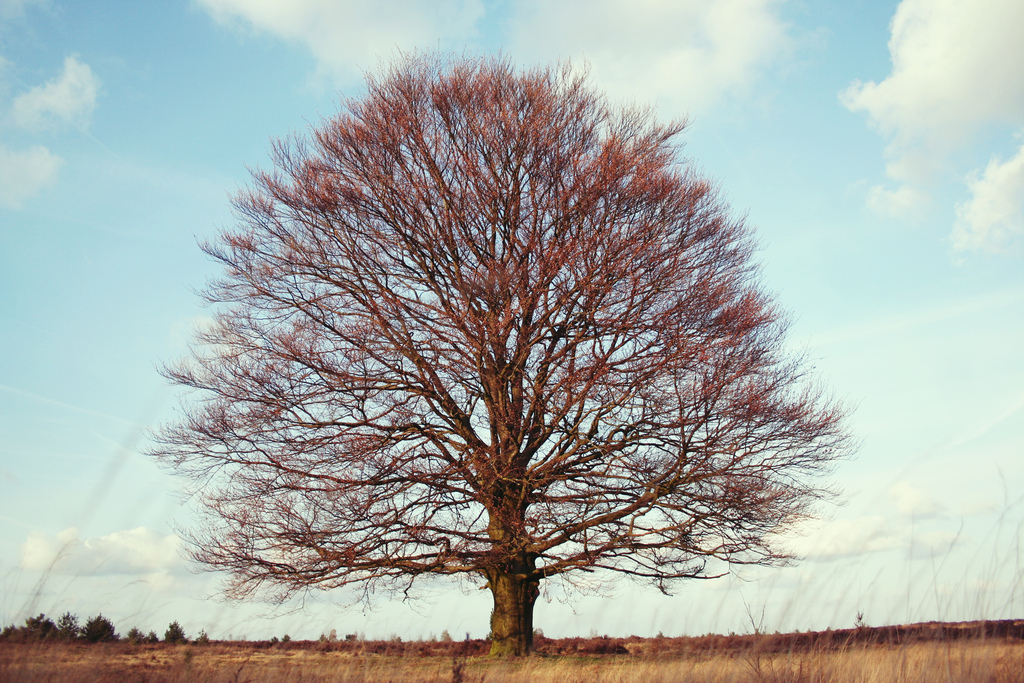
\includegraphics[width=\textwidth]{tree.jpeg}
  \end{columns}
\end{frame}
\addimgcredit{Tree: sxc.hu/bertvthul}
% -----------------------------------------------------------------------------
\begin{frame}
  \bigncentered{DEMO TIME}
\end{frame}
% }}}
% -----------------------------------------------------------------------------
\subsection{Scan}
% -----------------------------------------------------------------------------
% {{{
\begin{frame}{Scan}

  {\Huge
  \vspace*{-1cm}
  \begin{align*}
    y_1 &= x_1 \\
    y_2 &= f(y_1, x_2)\\
    \vdots &= \vdots \\
    y_N &= f(y_{N-1}, x_N)
  \end{align*}}
  where $N$ is the input size. (Think: $N$ large, $f(x,y)=x+y$)

  \begin{itemize}
    \item Prefix Sum/Cumulative Sum
    \item Abstract view of: loop-carried dependence
    \item Also possible: Segmented Scan
  \end{itemize}
\end{frame}
% -----------------------------------------------------------------------------
\begin{frame}{Scan: Graph}
  \begin{center}
    \begin{tikzpicture}[
      intermed/.style={input,fill=intermed},
      ffunc/.style={func,
        execute at end to={ node [left] {$f$}}
        },
      ]
      \foreach \i in {0,1,...,5}
      {
        \node [input] at (\i, 0) (x\i) { $x_{\i}$ };
        \node [output] at (\i, -6) (y\i) { $y_{\i}$ };
      }
      \foreach \i in {1,...,5}
      {
        \pgfmathtruncatemacro{\iminusone}{\i-1}
        \node [intermed] at (\i, -\i) (m\i) { $y_{\i}$ };
        \draw [func] (m\i) -- (y\i) node [pos=0.5,anchor=east] {Id};
        \draw [func] (x\i) -- (m\i) ;
      }
      \foreach \i in {2,...,5}
      {
        \pgfmathtruncatemacro{\iminusone}{\i-1}
        \draw [func] (m\iminusone) -- (m\i) ;
      }
      \draw [ffunc] (x0) -- (m1) ;
      \draw [func] (x0) -- (y0) node [pos=0.5,anchor=east] {Id};
    \end{tikzpicture}
  \end{center}
  \uncover<2->{
    \begin{tikzpicture} [overlay]
      \node [below left=1cm of current page.north east, draw,drop shadow,fill=white,
      text width=0.6\textwidth, inner xsep=0.5cm,inner ysep=0.5cm,thick]
        {
          This can't possibly be parallelized.

          Or can it?

          \only<3>{Again: Need assumptions on $f$.\\
          Associativity, commutativity.}
        } ;
    \end{tikzpicture}
  }
\end{frame}
% -----------------------------------------------------------------------------
\begin{frame}{Scan: Implementation}
  \begin{center}
    \begin{tikzpicture}[y=-1cm,scale=0.5]
      \foreach \i in {0,...,4}
      {
        \pgfmathtruncatemacro{\pwr}{2^\i}
        \pgfmathtruncatemacro{\nmpwr}{15-\pwr}
        \foreach \j in {0,...,15}
          \draw [fill=intermed,thick,draw] (\j,2*\i) rectangle +(1,1);
        \ifthenelse{\equal{\i}{4}}{}{
          \foreach \j in {\pwr,...,15}
            \draw [func] (\j,2*\i) ++(0.5,1) -- ++(0,1);
          \foreach \j in {0,...,\nmpwr}
            \draw [func] (\j,2*\i) ++(0.5,1) -- ++(\pwr,1);
        }
      }
    \end{tikzpicture}
  \end{center}
  \uncover<2->{
    \begin{tikzpicture} [overlay]
      \node [above left=1cm of current page.south east, draw,drop shadow,fill=white,
      inner xsep=0.5cm,inner ysep=0.5cm,thick]
        {
          Work-efficient?
        } ;
    \end{tikzpicture}
  }
\end{frame}
% -----------------------------------------------------------------------------
\begin{comment}
\begin{frame}{Scan: Implementation II}
  \begin{columns}
    \column{0.7\textwidth}
      Two sweeps: Upward, downward, \\
      both tree-shape

      \bigskip
      On upward sweep:
      \begin{itemize}
        \item Get values \texttt{L} and \texttt{R} from left and right child
        \item Save $L$ in local variable \texttt{Mine}
        \item Compute $\texttt{Tmp}=\texttt{L}+\texttt{R}$
          and pass to parent
      \end{itemize}

      On downward sweep:
      \begin{itemize}
        \item Get value $\texttt{Tmp}$ from parent
        \item Send $\texttt{Tmp}$ to left child
        \item Sent $\texttt{Tmp+Mine}$ to right child
      \end{itemize}
    \column{0.3\textwidth}
      \begin{tikzpicture}[
      grow=up,
      every node/.style={circle,fill=intermed,draw,thick, minimum width=0.4cm},
      every path/.style={func,<-},
      level distance=0.75cm,
      level 1/.style={sibling distance=1cm},
      level 2/.style={sibling distance=0.5cm},
      ]
        \node {}
        child {
          node {}
          child { node {} }
          child { node {} }
        }
        child {
          node {}
          child { node {} }
          child { node {} }
        }
        ;
      \end{tikzpicture}

      \bigskip
      \begin{tikzpicture}[
      grow=down,
      every node/.style={circle,fill=intermed,draw,thick, minimum width=0.4cm},
      every path/.style={func,->},
      level distance=0.75cm,
      level 1/.style={sibling distance=1cm},
      level 2/.style={sibling distance=0.5cm},
      ]
        \node {}
        child {
          node {}
          child { node {} }
          child { node {} }
        }
        child {
          node {}
          child { node {} }
          child { node {} }
        }
        ;
      \end{tikzpicture}
  \end{columns}
  \uncover<2->{
    \begin{tikzpicture} [overlay]
      \node [above left=1cm of current page.south east, draw,drop shadow,fill=white,
      text width=0.6\textwidth,inner xsep=0.5cm,inner ysep=0.5cm,thick]
        {
          Work-efficient?

          %Span rel. to first attempt?
        } ;
    \end{tikzpicture}
  }
\end{frame}
\end{comment}
% -----------------------------------------------------------------------------
\begin{frame}{Scan: Examples}
  \begin{columns}
    \column{0.6\textwidth}

      Low-level building block for many higher-level algorithms
      algorithms

      \begin{itemize}
        \item Index computations (!)
          \subitem{E.g. sorting}
        \item Anything with a loop-carried dependence
        %\item One row of Gauss-Seidel
        \item One row of triangular solve
        \item Segment numbering if boundaries are known
        \item FIR/IIR Filtering
        \item G.E.~Blelloch:
        \weblink{http://www.cs.cmu.edu/~guyb/papers/Ble93.pdf}{Prefix Sums and their Applications}
      \end{itemize}

    \column{0.3\textwidth}
      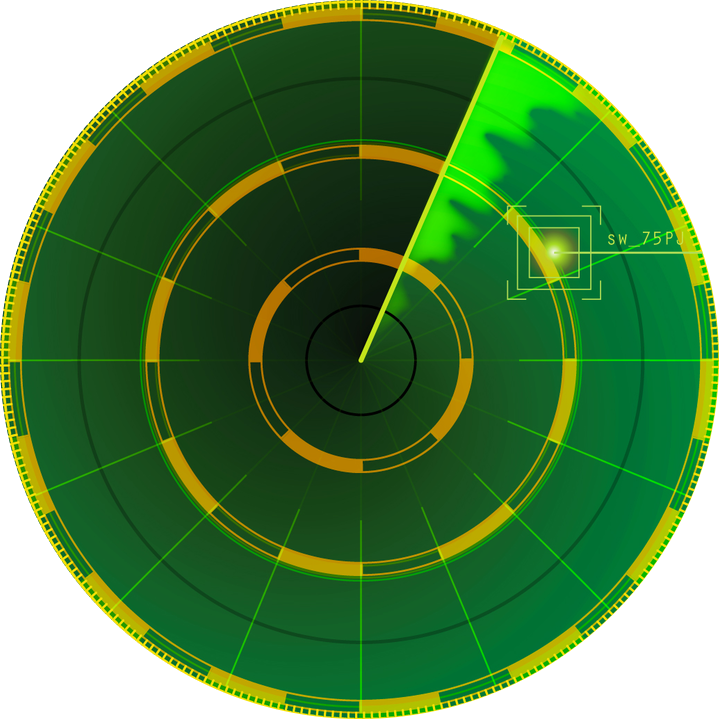
\includegraphics[width=\textwidth]{radar.png}
  \end{columns}
\end{frame}
\addimgcredit{Radar: sxc.hu/KimPouss}
% -----------------------------------------------------------------------------
\begin{frame}{Scan: Issues}
  \begin{columns}
    \column{0.3\textwidth}
      
\includegraphics[width=\textwidth]{question-mark.png}
    \column{0.6\textwidth}
      \begin{itemize}
        \item Subtlety: Inclusive/Exclusive Scan
        \item Pattern sometimes hard to recognize
          \begin{itemize}
            \item But shows up surprisingly often
            \item Need to prove associativity/commutativity
          \end{itemize}
        %\item Useful in Implementation: algorithm cascading
          %\subitem{Do sequential scan on parts, then parallelize at
          %coarser granularities}
      \end{itemize}
  \end{columns}
\end{frame}
% -----------------------------------------------------------------------------
\begin{frame}
  \bigncentered{DEMO TIME}
\end{frame}
% -----------------------------------------------------------------------------
\begin{frame}{Scan: Features}
  \begin{columns}
    \column{0.6\textwidth}
    \begin{itemize}
      \item ``Map'' processing on input: $f(x_i)$
        \subitem{Also: stencils $f(x_{i-1}, x_i)$}
      \item ``Map'' processing on output
        \begin{itemize}
          \item Output stencils
          \item Inclusive/Exclusive scan
        \end{itemize}
      \item Segmented scan
      \item Works on compound types
      \item Efficient!
    \end{itemize}
    \column{0.4\textwidth}
      \colorlet{input}{green!30}
      \colorlet{output}{red!30}
      \colorlet{intermed}{blue!30}

      \tikzset{
        input/.style={circle,fill=input,draw,thick},
        output/.style={circle,fill=output,draw,thick},
        func/.style={->,thick},
      }
      \begin{tikzpicture}[
        scale=0.5,
        intermed/.style={input,fill=intermed},
        ffunc/.style={func,
          execute at end to={ node [left] {$f$}}
          },
        ]
        \foreach \i in {0,1,...,5}
        {
          \node [input] at (\i, 0) (x\i) {  };
          \node [output] at (\i, -6) (y\i) {  };
        }
        \foreach \i in {1,...,5}
        {
          \pgfmathtruncatemacro{\iminusone}{\i-1}
          \node [intermed] at (\i, -\i) (m\i) { };
          \draw [func] (m\i) -- (y\i) ;
          \draw [func] (x\i) -- (m\i) ;
        }
        \foreach \i in {2,...,5}
        {
          \pgfmathtruncatemacro{\iminusone}{\i-1}
          \draw [func] (m\iminusone) -- (m\i) ;
        }
        \draw [ffunc] (x0) -- (m1) ;
        \draw [func] (x0) -- (y0) ;
      \end{tikzpicture}
  \end{columns}
  \uncover<+->{}
  \uncover<+->{
    \begin{tikzpicture} [overlay]
      \node [above left=7mm of current page.south east,
      draw,drop shadow,fill=white,inner sep=5mm,thick,
      text width=0.6\textwidth]
        {
          Scan: a \textbf{fundamental} parallel primitive.

          \bigskip

          Anything involving index changes/renumbering!

          (e.g. sort, filter, \dots)
        } ;
    \end{tikzpicture}
  }
\end{frame}
% -----------------------------------------------------------------------------
\begin{frame}{Scan: More Algorithms}
  \begin{itemize}
    \item \texttt{copy\_if}
    \item \texttt{remove\_if}
    \item \texttt{partition}
    \item \texttt{unique}
    \item \texttt{sort} (plain and key-value)
    \item \texttt{build\_list\_of\_lists}
    \item \texttt{bin\_sort}
  \end{itemize}
  All in \texttt{pyopencl}, all built on scan.
\end{frame}
% }}}

% }}}
\appendix
% -----------------------------------------------------------------------------
\section[Runtime]{OpenCL runtime}
% -----------------------------------------------------------------------------
\subsection{A Kingdom of Nouns}
% -----------------------------------------------------------------------------
% {{{
\begin{frame}{OpenCL Object Diagram}
  \begin{center}
  
\includegraphics[viewport=1.2in 4in 8.5in 10in,clip=true,page=20,height=0.7\textheight]{opencl-11.pdf}
  \end{center}
  \creditto{Credit: Khronos Group}
\end{frame}

\begin{frame}{CL ``Platform''}
  \begin{columns}
    \column{0.25\textwidth}
      \begin{tikzpicture}[x=1cm,y=2cm]
        \foreach \i in {1,...,10}
        {
          \pgfmathrand
          \let\myx=\pgfmathresult
          \pgfmathrand
          \let\myy=\pgfmathresult
          \node at (\myx, \myy) {
            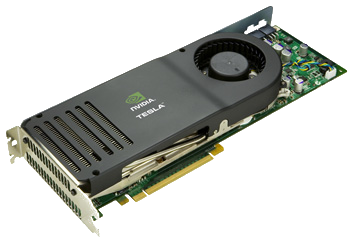
\includegraphics[width=0.6\textwidth]{c870.png}
          } ;
        }
      \end{tikzpicture}
    \column{0.75\textwidth}
    \begin{itemize}
      \item ``Platform'': a collection of devices, all from 
        the same \emph{vendor}.

      \item All devices in a platform use same CL driver/implementation.
      \item Multiple platforms can be used from one
        program $\rightarrow$ \emph{ICD}.

        \medskip
        \texttt{libOpenCL.so}: ICD loader

        \medskip
        \texttt{/etc/OpenCL/vendors/\textit{somename}.icd}:
          Plain text file with name of \texttt{.so} containing 
          CL implementation.

    \end{itemize}
  \end{columns}
\end{frame}

\begin{frame}{CL ``Compute Device''}
  \begin{columns}
    \column{0.25\textwidth}
      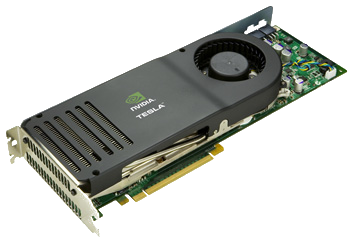
\includegraphics[width=\textwidth]{c870.png}
    \column{0.75\textwidth}
      CL Compute Devices:
      \begin{itemize}
        \item CPUs, GPUs, accelerators, \dots
          \subitem{Anything that fits the programming model.}
        \item A processor die with an interface to off-chip memory
        \item Can get list of devices from platform.
      \end{itemize}
  \end{columns}
\end{frame}


\begin{frame}[fragile]{Contexts}
  \begin{lstlisting}[gobble=4]
    context = cl.Context(devices=None | [dev1, dev2], dev_type=None)
    context = cl.create_some_context(interactive=True)
  \end{lstlisting}

  \begin{columns}
    \column{0.25\textwidth}
      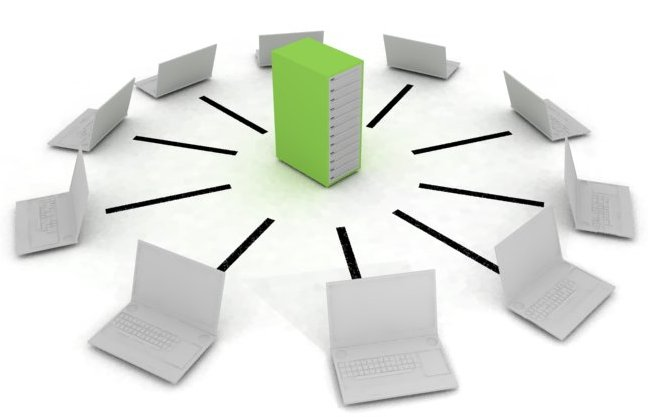
\includegraphics[width=\textwidth]{context.jpeg}
    \column{0.75\textwidth}
      \begin{itemize}
        \item Spans one or more Devices
        \item Create from device type or list of devices
          \subitem{See docs for \texttt{cl.Platform}, \texttt{cl.Device}}
        \item \texttt{dev\_type}: 
          \texttt{\textit{DEFAULT}},
          \texttt{ALL}, \texttt{CPU}, \texttt{GPU}
        \item Needed to\dots
          \begin{itemize}
            \item \dots allocate Memory Objects
            \item \dots create and build Programs
            \item \dots host Command Queues
            \item \dots execute Grids
          \end{itemize}
      \end{itemize}
  \end{columns}
\end{frame}
\addimgcredit{Context: sxc.hu/svilen001}


{
  \newcommand{\brick}[6]{
    \draw [fill=#4!50]
      (0,0) rectangle (#1,#2) coordinate [pos=0.5] (brickfront);
    \draw [fill=#4]
      (#1,0) -- (#1,0,-1) -- (#1,#2,-1) -- (#1,#2) --cycle;
    \draw [fill=#4]
      (0,#2) -- (0,#2,-1) -- (#1,#2,-1) -- (#1,#2) --cycle;
    #6
    \begin{pgfonlayer}{foreground}
      \node [fill=#4!50,inner xsep=2pt,inner ysep=2pt,opacity=0.7,#5] at (brickfront) { #3 } ;
      \node [#5] at (brickfront) { #3 } ;
    \end{pgfonlayer}
  }
  \newcommand{\drawevt}[2]{
    \fill [#2,opacity=0.5] 
      (0,#1) -- (1.5,#1) -- (1.5,#1,-1)
      -- (1.5,#1+0.2,-1) -- (1.5,#1+0.2) -- (0,#1+0.2) --  cycle ;
  }
  \begin{frame}{OpenCL: Command Queues}
    \begin{columns}
      \column{0.45\textwidth}
        \begin{itemize}
          \item Host and Device run asynchronously
          \item Host submits to queue:
            \uncover{
              \begin{itemize}
                \item Computations
                \item Memory Transfers
                \item Sync primitives
                \item \dots
              \end{itemize}
            }
          \item Host can wait for\\drained queue
          \item Profiling

        \end{itemize}

      \column{0.5\textwidth}
        \begin{tikzpicture}
          \brick{1.25}{2}{Host}{gray}{}{}
          \begin{scope}[xshift=2.5cm,yshift=-1.5cm]
            \brick{2.5}{1.25}{Device}{gray}{}{}
          \end{scope}
          \begin{scope}[xshift=2.5cm]
            \brick{0.75}{2}{Queue 1}{blue}{text=white,rotate=90}{
              \foreach\i in {0,0.2,...,1.4}
                \draw (0,\i) -- (0.75,\i) -- (0.75,\i,-1);
            }
          \end{scope}
          \begin{scope}[xshift=3.5cm]
            \brick{0.75}{2}{Queue 2}{blue}{text=white,rotate=90}{
              \foreach\i in {0,0.2,...,0.9}
                \draw (0,\i) -- (0.75,\i) -- (0.75,\i,-1);
            }
          \end{scope}

          \node [font=\Large] at (5.25,1.25) {\dots} ;

          \draw [very thick,->] (1.25,1,-0.5) -| (2,2.5,-0.5) -| (2.875,2,-0.5);
          \draw [very thick,->] (2,2.5,-0.5) -| (3.875,2,-0.5);
          \draw [very thick,->] (2,2.5,-0.5) -| (4.875,2,-0.5);
          \draw [very thick,->] (2.5,-1) -| (0.625,0);
            
        \end{tikzpicture}
    \end{columns}
  \end{frame}
}

\begin{frame}[fragile]{Command Queues and Events}
  \begin{lstlisting}[gobble=4]
    queue = cl.CommandQueue(context, device=None, 
      properties=None | [(prop, value),...])
  \end{lstlisting}
  \begin{columns}
    \column{0.65\textwidth}
        \begin{itemize}
          \item Attached to single device
          \item \text{cl.command\_queue\_properties}\dots
            \begin{itemize}
              \item \texttt{OUT\_OF\_ORDER\_EXEC\_MODE\_ENABLE}:\\
                Do not force sequential execution
              \item \texttt{PROFILING\_ENABLE}:\\
                Gather timing info
            \end{itemize}
        \end{itemize}
    \column{0.35\textwidth}
      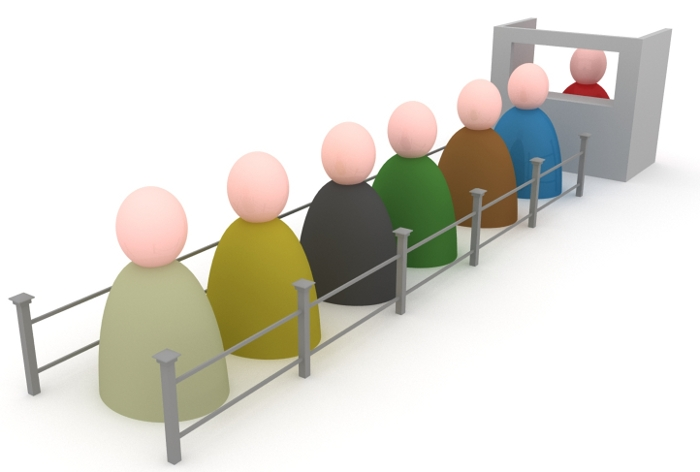
\includegraphics[width=\textwidth]{queue.jpeg}
  \end{columns}
\end{frame}
\addimgcredit{Queue: sxc.hu/cobrasoft}



\begin{frame}{Capturing Dependencies}
  \begin{columns}
    \column{0.3\textwidth}
      B = f(A)\\
      C = g(B)\\
      E = f(C)\\
      F = h(C)\\
      G = g(E,F)\\
      P = p(B)\\
      Q = q(B)\\
      R = r(G,P,Q)
    \column{0.6\textwidth}
      \begin{center}
        \begin{tikzpicture}[
  scale=0.014,thick,
  annode/.style={xshift=0.1cm},
  intermed/.style={input,fill=intermed},
  ]
    \node [input] (A) at (152,479) [draw,ellipse] {A};
    \node [intermed] (C) at (80,295) [draw,ellipse] {C};
    \node [intermed] (B) at (152,387) [draw,ellipse] {B};
    \node [intermed] (E) at (27,203) [draw,ellipse] {E};
    \node [intermed] (G) at (99,111) [draw,ellipse] {G};
    \node [intermed] (F) at (99,203) [draw,ellipse] {F};
    \node [intermed] (Q) at (211,203) [draw,ellipse] {Q};
    \node [intermed] (P) at (152,295) [draw,ellipse] {P};
    \node [output] (R) at (154,19) [draw,ellipse] {R};
    \draw [->] (C) -- (F);
    \draw (96,249) node [annode] {h};
    \draw [->] (G) -- (R);
    \draw (134.5,65) node [annode] {r};
    \draw [->] (B) -- (C);
    \draw (126.5,341) node [annode] {g};
    \draw [->] (P) -- (R);
    \draw (156.5,157) node [annode] {r};
    \draw [->] (E) -- (G);
    \draw (73.5,157) node [annode] {g};
    \draw [->] (Q) -- (R);
    \draw (193.5,111) node [annode] {r};
    \draw [->] (F) -- (G);
    \draw (103.5,157) node [annode] {g};
    \draw [->] (B) -- (Q);
    \draw (202.5,295) node [annode] {q};
    \draw [->] (A) -- (B);
    \draw (154.5,433) node [annode] {f};
    \draw [->] (B) -- (P);
    \draw (156.5,341) node [annode] {p};
    \draw [->] (C) -- (E);
    \draw (61.5,249) node [annode] {f};
\end{tikzpicture}

      \end{center}
  \end{columns}
  \uncover<2>{
    \begin{tikzpicture} [overlay]
      \node [above right=1cm of current page.south west, draw,drop shadow,fill=white,
      text width=0.6\textwidth, inner xsep=0.5cm,inner ysep=0.5cm,thick]
        {
          \begin{itemize}
            \item Switch queue to out-of-order mode!

            \item Specify as list of events using 
              \texttt{wait\_for=} optional keyword
              to \texttt{enqueue\_XXX}.

            \item Can also enqueue barrier.

            \item Common use case: Transmit/receive
              from other MPI ranks.

            \item Possible in hardware on Nv Fermi, AMD Cayman:
              Submit parallel work to increase machine use.
              \subitem{Not yet ubiquitously implemented}
          \end{itemize}
        } ;
    \end{tikzpicture}
  }
\end{frame}

\begin{frame}[fragile]{Memory Objects: Buffers}
  \begin{lstlisting}[gobble=4]
    buf = cl.Buffer(context, flags, size=0, hostbuf=None)
  \end{lstlisting}
  \begin{columns}
    \column{0.7\textwidth}
      \begin{overlayarea}{\textwidth}{0.7\textheight}
        \only<+>{
          \begin{itemize}
            \item Chunk of device memory
            \item No type information: ``Bag of bytes''
            \item Observe: \emph{Not} tied to device.

              $\rightarrow$ no fixed memory address

              $\rightarrow$ pointers do \emph{not} survive kernel
              launches

              $\rightarrow$ movable between devices

              $\rightarrow$ not even allocated before first use!
            \item \texttt{flags}:
              \begin{itemize}
                \item \texttt{READ\_ONLY/WRITE\_ONLY/READ\_WRITE}
                \item \{\texttt{ALLOC,COPY,USE}\}\texttt{\_HOST\_PTR}
              \end{itemize}
          \end{itemize}
        }
        \only<+>{
          \texttt{COPY\_HOST\_PTR}:
          \begin{itemize}
            \item Use \texttt{hostbuf} as initial content of buffer
          \end{itemize}
          \texttt{USE\_HOST\_PTR}:
          \begin{itemize}
            \item \texttt{hostbuf} \emph{is} the buffer. 
            \item Caching in device memory is allowed.
          \end{itemize}
          \texttt{ALLOC\_HOST\_PTR}:
          \begin{itemize}
            \item \emph{New} host memory (unrelated to
              \texttt{hostbuf}) is visible from device
              \emph{and} host.
          \end{itemize}
        }
        \only<+>{
          \begin{itemize}
            \item Specify \texttt{hostbuf} or \texttt{size} (or both)
            \item \texttt{hostbuf}: Needs Python Buffer Interface\\
              e.g. \texttt{numpy.ndarray}, \texttt{str}.
              \subitem{Important: Memory layout matters}
            \item Passed to device code as pointers\\
              (e.g. \texttt{float *}, \texttt{int *})
            \item \texttt{enqueue\_copy}(queue, dest, src)
            \item Can be mapped into host address space:\\
              \texttt{cl.MemoryMap}.
          \end{itemize}
        }
      \end{overlayarea}
    \column{0.3\textwidth}
      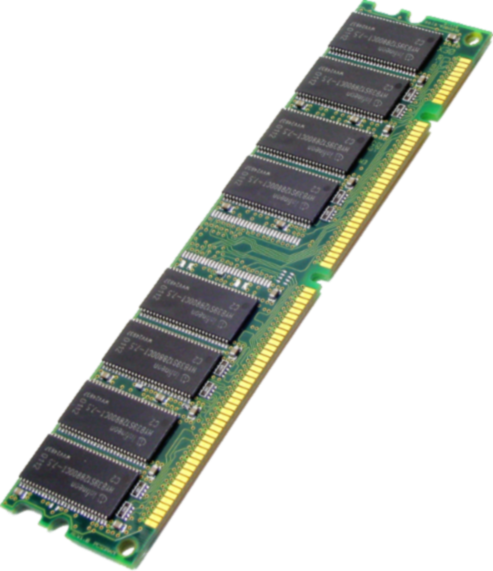
\includegraphics[width=\textwidth]{memory.png}
  \end{columns}
\end{frame}
\addimgcredit{RAM stick: sxc.hu/gobran11}

\begin{frame}[fragile]{Programs and Kernels}
  \begin{lstlisting}[gobble=4]
    prg = cl.Program(context, src)
  \end{lstlisting}
  \begin{columns}
    \column{0.65\textwidth}
      \begin{itemize}
        \item \texttt{src}: OpenCL device code
          \begin{itemize}
            \item Derivative of C99
            \item Functions with \texttt{\_\_kernel} attribute
              can be invoked from host
          \end{itemize}
        \item \texttt{prg.build(options="",\\
          \hspace*{2em}devices=None)}
        \item \texttt{kernel = prg.kernel\_name}
        \item \texttt{kernel(queue,\\
          \hspace*{2em}$(G_x,G_y,G_z)$, $(L_x,L_y,L_z)$, \\
          \hspace*{2em}arg, \dots, \\
          \hspace*{2em}wait\_for=None)}\\
      \end{itemize}
    \column{0.3\textwidth}
      % boo yuck
      \hspace*{-1cm}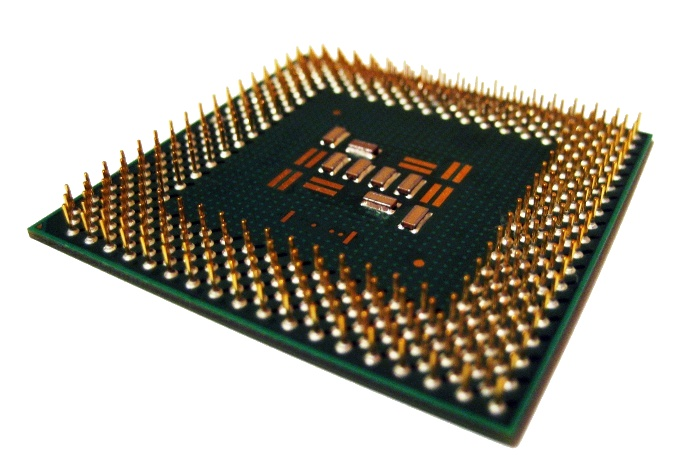
\includegraphics[width=1.3\textwidth]{cpu.jpeg}
  \end{columns}
\end{frame}
\begin{frame}[fragile]{Program Objects}
  \begin{lstlisting}[gobble=4]
    kernel(queue, (Gx,Gy,Gz), (Sx,Sy,Sz), arg, ..., wait_for=None)
  \end{lstlisting}
  \begin{columns}
    \column{0.3\textwidth}
      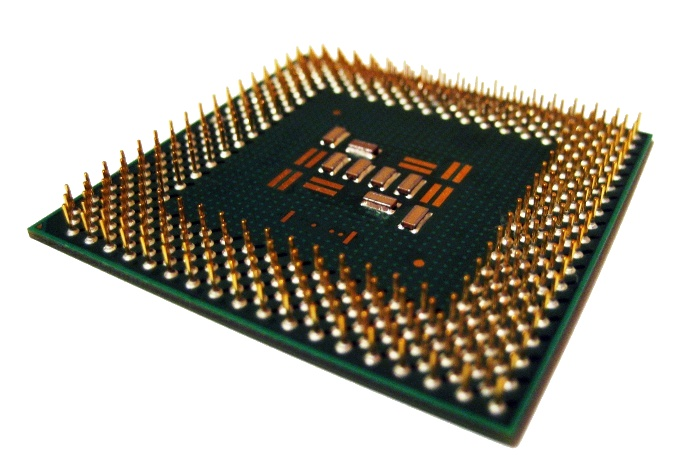
\includegraphics[width=1.3\textwidth]{cpu.jpeg}
    \column{0.65\textwidth}
      \begin{overlayarea}{\textwidth}{0.5\textheight}
        \only<+>{
          \texttt{arg} may be:
          \begin{itemize}
            \item \texttt{None} (a \texttt{NULL} pointer)
            \item \texttt{numpy} sized scalars:
              \texttt{numpy.int64,numpy.float32,\dots}
            \item Anything with buffer interface:\\
              \texttt{numpy.ndarray}, \texttt{str}\\
            \item Buffer Objects
            \item Also: \texttt{cl.Image}, \texttt{cl.Sampler}, 
              \texttt{cl.LocalMemory}
          \end{itemize}
        }
        \only<+>{
          Explicitly sized scalars:\\
          {\color{red}\ding{54}  Annoying, error-prone.}

          \medskip
          Better:

          \texttt{%
          kernel.set\_scalar\_arg\_dtypes([\\
          \hspace*{3ex}numpy.int32, None,\\
          \hspace*{3ex}numpy.float32])}
          \medskip

          Use \texttt{None} for non-scalars.
        }
      \end{overlayarea}
  \end{columns}
\end{frame}
\addimgcredit{CPU: sxc.hu/dimshik}


\begin{frame}{OpenCL Object Diagram}
  \begin{center}
  
\includegraphics[viewport=1.2in 4in 8.5in 10in,clip=true,page=20,height=0.7\textheight]{opencl-11.pdf}
  \end{center}
  \creditto{Credit: Khronos Group}
\end{frame}
% }}}
% -----------------------------------------------------------------------------
\subsection{Synchronization}
% -----------------------------------------------------------------------------
% {{{
\begin{nologo}
\begin{frame}{Recap: Concurrency and Synchronization}
  \uncover<+->{
    \begin{beamercolorbox}[sep=3mm]{block body}
      GPUs have layers of concurrency.\\
      \hfill Each layer has its synchronization primitives.
    \end{beamercolorbox}
  }
  \bigskip
  \begin{columns}[c]
    \column{0.6\textwidth}
      \uncover<+->{
        \begin{itemize}
          \item Intra-group:\\ 
            \texttt{barrier(\dots)}, \\
            %\texttt{mem\_fence(\dots)}\\
            \texttt{\dots} =
            \texttt{CLK\_\{LOCAL,GLOBAL\}\_MEM\_FENCE}
          \item Inter-group:\\ Kernel launch
          \item CPU-GPU:\\ Command queues, Events
        \end{itemize}
      }
    \column{0.35\textwidth}
      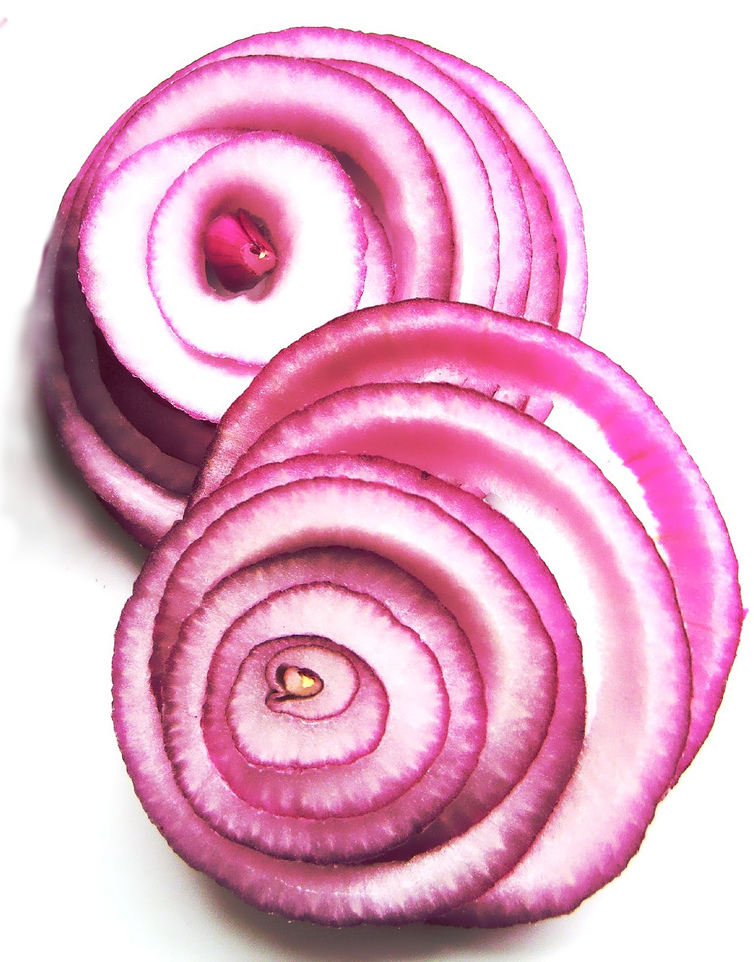
\includegraphics[width=\textwidth]{onion.jpeg}
  \end{columns}

\end{frame}
\end{nologo}
\addimgcredit{Onions: flickr.com/darwinbell \cc}
% -----------------------------------------------------------------------------
\begin{frame}{Synchronization between Groups}
  \begin{block}<+->{Golden Rule:}
    Results of the algorithm must be independent of the order in which
    work groups are executed.
  \end{block}

  \uncover<+->{%
  \textbf{Consequences:}
  \begin{itemize}
    \item Work groups may read the same information from global memory.
    \item But: Two work groups may not validly write different things to
      the same global memory.
    \item Kernel launch serves as
      \begin{itemize}
        \item Global barrier
        \item Global memory fence
      \end{itemize}
  \end{itemize}
  }
\end{frame}
\begin{frame}{Synchronization}
  What is a Barrier?

  \bigskip
  \begin{center}
  \begin{tikzpicture}[scale=0.8,
  thread/.style={blue,very thick,->},
  barrier/.style={ultra thick},
  stopped/.style={fill=red,shape=regular polygon,regular polygon sides=8},
  ]
  \draw [barrier] (0,0) -- +(4,0) ;
  \uncover<+>{
    \draw [thread] (1,5) -- +(0,-2) ;
    \draw [thread] (2,5) -- +(0,-3) ;
    \draw [thread] (3,5) -- +(0,-1) ;
  }
  \uncover<+>{
    \draw [thread] (1,5) -- +(0,-3) ;
    \draw [thread] (2,5) -- +(0,-4) ;
    \draw [thread] (3,5) -- +(0,-2) ;
  }
  \uncover<+>{
    \node [stopped] at (2,0) {};
    \draw [thread] (1,5) -- +(0,-4) ;
    \draw [thread] (2,5) -- +(0,-5) ;
    \draw [thread] (3,5) -- +(0,-3) ;
  }
  \uncover<+>{
    \node [stopped] at (2,0) {};
    \node [stopped] at (1,0) {};
    \draw [thread] (1,5) -- +(0,-5) ;
    \draw [thread] (2,5) -- +(0,-5) ;
    \draw [thread] (3,5) -- +(0,-4) ;
  }
  \uncover<+>{
    \node [stopped] at (2,0) {};
    \node [stopped] at (1,0) {};
    \node [stopped] at (3,0) {};
    \draw [thread] (1,5) -- +(0,-5) ;
    \draw [thread] (2,5) -- +(0,-5) ;
    \draw [thread] (3,5) -- +(0,-5) ;
  }
  \uncover<+>{
    \draw [thread] (1,5) -- +(0,-5) ;
    \draw [thread] (2,5) -- +(0,-5) ;
    \draw [thread] (3,5) -- +(0,-5) ;
  }
  \uncover<+>{
    \draw [thread] (1,5) -- +(0,-6) ;
    \draw [thread] (2,5) -- +(0,-6) ;
    \draw [thread] (3,5) -- +(0,-6) ;
  }
  \end{tikzpicture}
  \end{center}
\end{frame}


%\begin{frame}{Synchronization}
  What is a Memory Fence?

  \bigskip
  \begin{center}
  \begin{tikzpicture}[scale=0.8,
  thread/.style={blue,very thick,->},
  fence/.style={ultra thick},
  memlocation/.style={thick,draw,fill=blue!20,minimum width=1.5cm},
  write/.style={thick,->,red,dashed},
  read/.style={thick,->,green,dashed},
  meminstr/.style={pos=0.5,font=\small},
  ]
  \only<1-5>{
    \node [memlocation] (mem) at (0,1) { 17 } ;
  }
  \only<6-7>{
    \node [memlocation] (mem) at (0,1) { 18 } ;
  }
  \uncover<+-+(1)>{
    \draw [thread] (-3,5) -- +(0,-1) coordinate (t1write) ;
    \draw [thread] (3,5) -- +(0,-1) ;
  }
  \uncover<+-+(4)>{
    \draw [write] (t1write) -- (mem) node [meminstr] {write 18};
  }
  \uncover<+>{
    \draw [thread] (-3,5) -- +(0,-2) ;
    \draw [thread] (3,5) -- +(0,-2) coordinate (t2read);
  }
  \uncover<.-.(1)>{
    \draw [read] (t2read) -- (mem) node [meminstr] {read};
  }
  \uncover<+>{
    \draw [thread] (-3,5) -- +(0,-3) ;
    \draw [thread] (3,5) -- +(0,-3) coordinate (t2readc);
    \draw [read] (mem) -- (t2readc) node [meminstr] {17};
  }
  \uncover<+>{
    \draw [thread] (-3,5) -- +(0,-4) ;
    \draw [thread] (3,5) -- +(0,-4) ;
  }
  \uncover<+>{
    \draw [thread] (-3,5) -- +(0,-5) ;
    \draw [thread] (3,5) -- +(0,-5) ;
  }
  \uncover<+>{
    \draw [thread] (-3,5) -- +(0,-6) ;
    \draw [thread] (3,5) -- +(0,-6) ;
  }

  \end{tikzpicture}
  \end{center}
\end{frame}
% -----------------------------------------------------------------------------
\begin{frame}{Synchronization}
  What is a Memory Fence? An ordering restriction for memory access.

  \bigskip
  \begin{center}
  \begin{tikzpicture}[scale=0.8,
  thread/.style={blue,very thick,->},
  fence/.style={ultra thick},
  memlocation/.style={thick,draw,fill=blue!20,minimum width=1.5cm},
  write/.style={thick,->,red,dashed},
  read/.style={thick,->,green,dashed},
  meminstr/.style={pos=0.5,font=\small},
  stopped/.style={fill=red,shape=regular polygon,regular polygon sides=8},
  ]
  \draw [fence] (-4,0) -- (4,0) ;
  \only<1-4>{
    \node [memlocation] (mem) at (0,0) { 17 } ;
  }
  \only<5->{
    \node [memlocation] (mem) at (0,0) { 18 } ;
  }
  \uncover<+-+(1)>{
    \draw [thread] (-3,2) -- +(0,-1) coordinate (t1write) ;
    \draw [thread] (3,2) -- +(0,-1) ;
  }
  \uncover<+-+(2)>{
    \draw [write] (t1write) -- (mem) node [meminstr] {write 18};
  }
  \uncover<+-+(3)>{
    \draw [thread] (-3,2) -- +(0,-2) ;
    \draw [thread] (3,2) -- +(0,-2) coordinate (t2read);
  }
  \uncover<+-+(1)>{
    \node [stopped] at (-3,0) {};
    \node [stopped] at (3,0) {};
  }
  \addtocounter{beamerpauses}{2}

  \uncover<+>{
    \draw [thread] (-3,2) -- +(0,-3) ;
    \draw [thread] (3,2) -- +(0,-3) coordinate (t2read);
  }
  \uncover<.->{
    \draw [read] (t2read) -- (mem) node [meminstr] {read};
  }
  \uncover<+->{
    \draw [thread] (-3,2) -- +(0,-4) ;
    \draw [thread] (3,2) -- +(0,-4) coordinate (t2readc);
    \draw [read] (mem) -- (t2readc) node [meminstr] {18};
  }

  \end{tikzpicture}
  \end{center}
  %\uncover<+->{
    %Flavors: All \{reads, writes, accesses\} complete\\
    %before continuing.
  %}
\end{frame}


% }}}

% -----------------------------------------------------------------------------
\section[]{OpenCL implementations}
% -----------------------------------------------------------------------------
% {{{

\begin{frame}{The Nvidia CL implementation}
  \begin{columns}
    \column{0.4\textwidth}
      
\includegraphics[width=\textwidth]{nvidia.pdf}
    \column{0.7\textwidth}
      Targets only GPUs

      \medskip
      Notes:
      \begin{itemize}
        \item Nearly identical to CUDA
          \subitem{No native C-level JIT in CUDA ($\rightarrow$ PyCUDA)}
        \item Page-locked memory:\\
          Use \texttt{CL\_MEM\_ALLOC\_HOST\_PTR}.\\
          (Careful: double meaning)
      \end{itemize}
  \end{columns}
\end{frame}
\addimgcredit{Nvidia logo: Nvidia Corporation}
\begin{frame}{The Apple CL implementation}
  \begin{columns}
    \column{0.6\textwidth}
      Targets CPUs and GPUs

      \medskip
      General notes:
      \begin{itemize}
        \item Different header name\\
          \texttt{OpenCL/cl.h} instead of \texttt{CL/cl.h}\\
          Use \texttt{-framework OpenCL} for C access.
        \item Beware of imperfect compiler cache implementation\\
          (ignores include files)
      \end{itemize}
      CPU notes:
      \begin{itemize}
        \item One work item per processor
      \end{itemize}
      GPU similar to hardware vendor implementation.\\
      (New: Intel w/ Sandy Bridge)
    \column{0.2\textwidth}
      
\includegraphics[width=\textwidth]{apple-logo.pdf}
  \end{columns}
\end{frame}
\addimgcredit{Apple logo: Apple Corporation}

\begin{frame}{The AMD CL implementation}
  \begin{columns}
    \column{0.1\textwidth}
      
\includegraphics[height=\textwidth,angle=90]{amd-logo.pdf}
    \column{0.85\textwidth}
      Targets CPUs and GPUs (from both AMD and Nvidia)

      \medskip
      GPU notes:
      \begin{itemize}
        \item Wide SIMD groups (64)
        \item GCN: Vector \emph{and} scalar unit (previously VLIW4/5)
        \begin{itemize}
          \item \emph{very} flop-heavy machine
          \item $\rightarrow$ ILP and explicit SIMD
          %\item Non-vector memory coalescing only on Cayman+
        \end{itemize}
      \end{itemize}

      CPU notes:
      \begin{itemize}
        \item Many work items per processor (emulated)
        \item ``APU'': Growing CPU/GPU integration
      \end{itemize}
  \end{columns}
\end{frame}
\addimgcredit{AMD logo: AMD Corporation}

\begin{frame}{The Intel CL implementation}
  \begin{columns}
    \column{0.75\textwidth}
      CPUs, GPUs with Ivy Bridge+

      \medskip
      CPU notes:
      \begin{itemize}
        \item Good vectorizing compiler
        \item Only implementation of out-of-order queues for now
        \item Based on Intel TBB
      \end{itemize}
      GPU notes:
      \begin{itemize}
        \item Flexible design: SIMD$m$ VLIW$n$
        \item Lots of fixed-function hardware
        \item Last-level Cache (LLC) integrated between CPU and GPU
      \end{itemize}

    \column{0.25\textwidth}
      
\includegraphics[width=\textwidth]{intel-logo.pdf}
  \end{columns}
\end{frame}
\addimgcredit{Intel logo: Intel Corporation}
% }}}

% }}}
\end{document}

% vim: foldmethod=marker
